% 建议使用 XeLaTeX 或 LuaLaTeX 编译(中文与公式支持更佳)
\documentclass[UTF8,zihao=-4]{ctexart}

\usepackage[a4paper,margin=2.5cm]{geometry}
\usepackage{amsmath, amssymb, amsthm}
\usepackage{bm}
\usepackage{hyperref}
\usepackage{graphicx}
\usepackage{caption}
\usepackage{listings}
\usepackage{xcolor}
\usepackage{float}
\usepackage{placeins}
\graphicspath{{figures/}}

\lstdefinestyle{code}{
  basicstyle=\ttfamily\small,
  numbers=left,
  numberstyle=\tiny,
  numbersep=8pt,
  keywordstyle=\color{blue},
  commentstyle=\color{teal!70!black},
  stringstyle=\color{orange!70!black},
  showstringspaces=false,
  breaklines=true,
  frame=single,
  framerule=0.3pt,
  rulecolor=\color{black!15}
}
\lstset{style=code}

\title{优势演员-评论家(A2C):原理、公式、应用与实战}
\author{}
\date{\today}

\begin{document}
\maketitle

\section{引言}
优势演员-评论家(Advantage Actor-Critic,A2C)是同步版的 Actor-Critic 架构。策略网络(Actor)根据优势函数的梯度进行更新,价值网络(Critic)提供低方差的价值估计,实现了稳定的策略梯度学习,并便于批量并行采样。

\section{原理与公式}
\subsection{Actor-Critic 目标}
给定策略 \(\pi_\theta(a\mid s)\) 与价值函数 \(V_w(s)\),策略梯度使用优势函数 \(A^{\pi}(s,a) = Q^{\pi}(s,a) - V^{\pi}(s)\):
\begin{equation}
\nabla_\theta J(\theta) = \mathbb{E}_{s,a}\big[ \nabla_\theta \log \pi_\theta(a\mid s)\, A^{\pi}(s,a) \big].
\end{equation}
时间差分(TD)误差提供优势的低方差估计。

\subsection{Critic 更新}
评论家最小化平方 TD 误差:
\begin{equation}
\delta_t = r_{t+1} + \gamma V_w(s_{t+1}) - V_w(s_t), \qquad V(s_t) \leftarrow V(s_t) + \beta \delta_t.
\end{equation}
在表格设定下直接更新值表;函数逼近时按梯度下降调整参数。

\subsection{Actor 更新}
Actor 使用相同的 TD 误差作为优势估计做梯度上升:
\begin{equation}
\theta \leftarrow \theta + \alpha \delta_t \nabla_\theta \log \pi_\theta(a_t\mid s_t).
\end{equation}
实际实现常加入熵正则 \(H[\pi_\theta(\cdot\mid s)]\) 以促进探索,并在多个环境间同步梯度。

\section{应用与技巧}
\begin{itemize}
  \item \textbf{离散控制}:GridWorld、Atari 等同步采样任务。
  \item \textbf{多环境并行}:利用向量化模拟器降低方差。
  \item \textbf{低延迟机器人}:当可在线更新且需要稳定性时。
  \item \textbf{实用建议}:对优势做标准化,调节熵系数,分别监控 Actor/Critic 损失,并通过梯度裁剪保持值函数稳定。
\end{itemize}

\section{Python 实战}
脚本 \texttt{gen\_a2c\_figures.py} 在线网格世界上训练表格型 A2C,展示回报曲线与学习到的价值函数热力图。
\begin{lstlisting}[language=Python,caption={脚本 gen_a2c_figures.py 片段}]
prob = softmax(theta[state])
action = rng.choice(n_actions, p=prob)
next_state, reward, done = env.step(state, action)
td_error = reward + gamma * V[next_state] * (1.0 - float(done)) - V[state]
V[state] += critic_lr * td_error
theta[state] += actor_lr * td_error * (one_hot(action, n_actions) - prob)
\end{lstlisting}

\section{实验结果}
\begin{figure}[H]
  \centering
  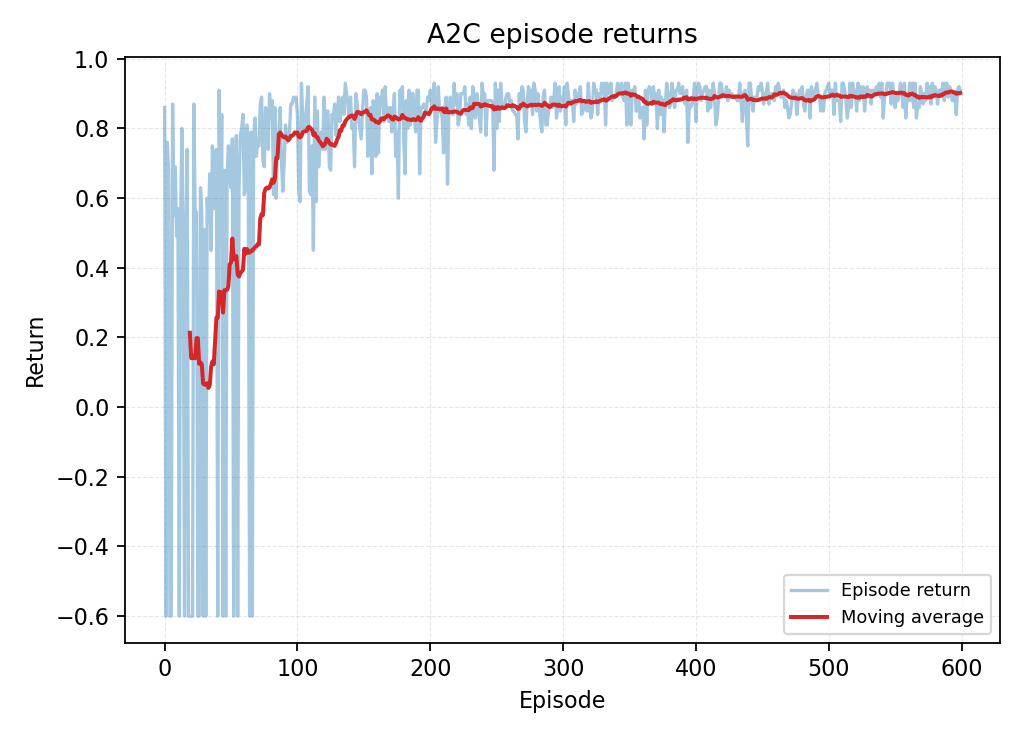
\includegraphics[width=0.8\linewidth]{a2c_returns.png}
  \caption{A2C 训练过程中的回报曲线及滑动平均}
  \label{fig:a2c_returns_cn}
\end{figure}

\begin{figure}[H]
  \centering
  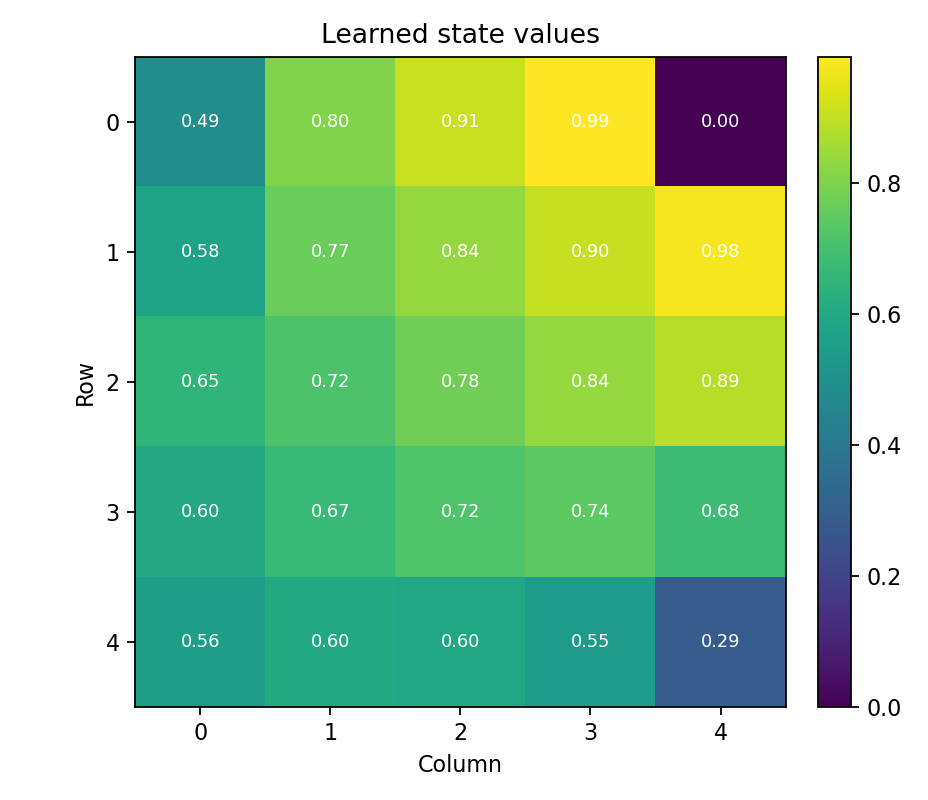
\includegraphics[width=0.82\linewidth]{a2c_value_baseline.png}
  \caption{评论家学习到的价值函数热力图,体现最优路径}
  \label{fig:a2c_value_baseline_cn}
\end{figure}

\FloatBarrier
\section{总结}
A2C 通过同步更新 Actor 与 Critic 降低策略梯度的方差并提高稳定性。适度的批量采样、优势归一化与熵正则是成功应用的关键。示例展示了回报逐步提升及价值函数如何编码最短路径结构。

\end{document}